\documentclass{beamer}
\usetheme{Madrid}
\usecolortheme{seahorse}

\title{Reservoir Computing: Implementation and Analysis}
\subtitle{Study Oriented Project}
\author{Vimarsh Shah\\Department of Physics, BITS Pilani Goa\\\texttt{f20221060@goa.bits-pilani.ac.in}}
\date{April 2025}
\institute{BITS Pilani, KK Birla Goa Campus}

\begin{document}

% Title Slide
\begin{frame}
  \titlepage
  \begin{center}
    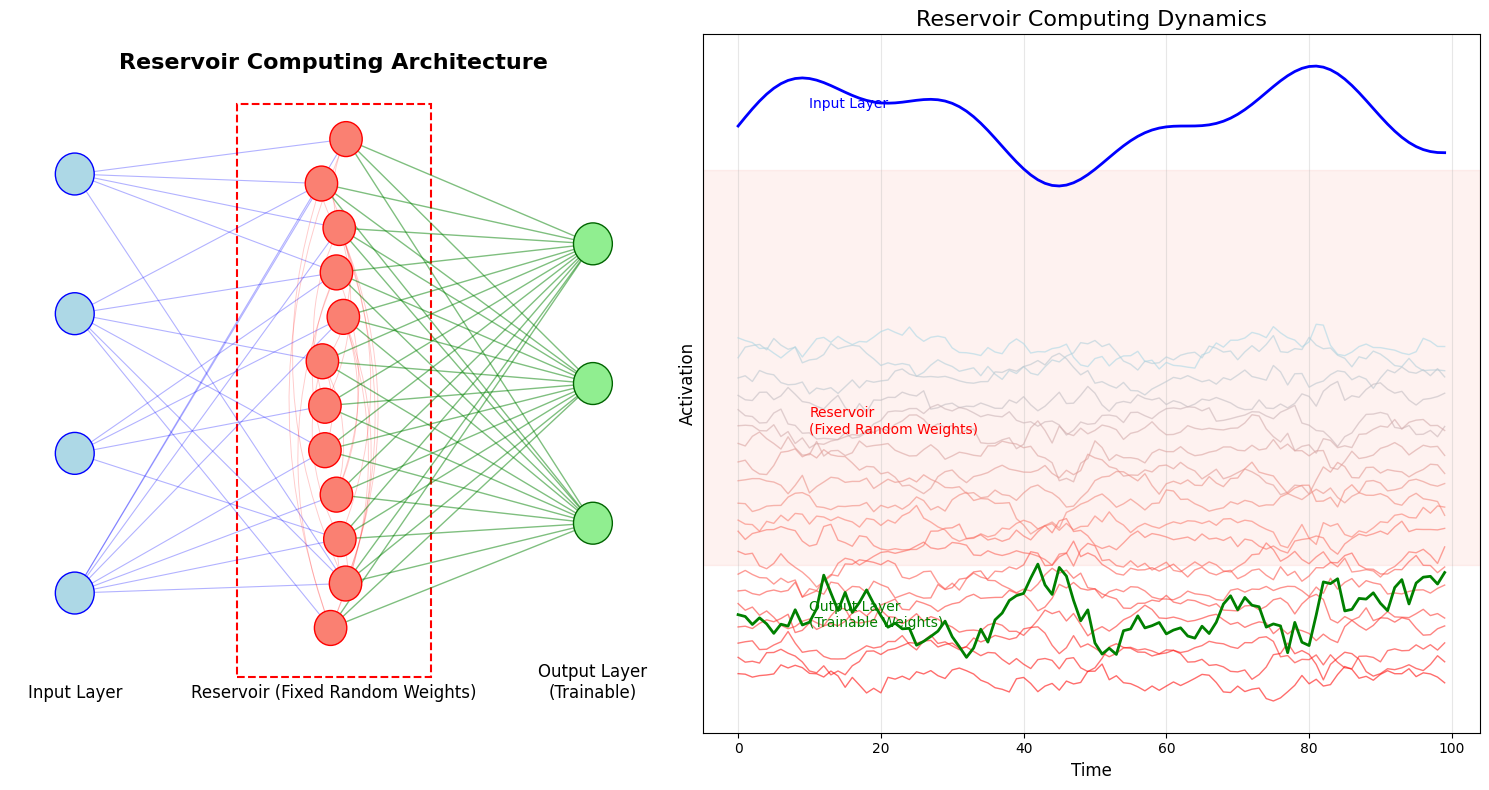
\includegraphics[width=0.7\linewidth]{ivt-style/rc_intro_matplotlib}
  \end{center}
\end{frame}

% Outline
\begin{frame}{Outline}
  \tableofcontents
\end{frame}

% Introduction
\section{Introduction}
\begin{frame}{Introduction}
  \begin{itemize}
    \item Machine learning enables pattern extraction and prediction from data.
    \item Traditional deep learning uses backpropagation, but RNNs face vanishing/exploding gradients.
    \item Reservoir Computing (RC) simplifies training by fixing the recurrent network and only training the output.
    \item RC is efficient for temporal modeling.
  \end{itemize}
\end{frame}

\begin{frame}{Motivation}
  \begin{itemize}
    \item RC maintains RNN representational power with easier training.
    \item Key advantages:
      \begin{itemize}
        \item Only output layer is trained (linear regression).
        \item Lower computational cost.
        \item Reservoir retains memory of past inputs.
        \item Can be implemented physically.
      \end{itemize}
  \end{itemize}
\end{frame}

\begin{frame}{Neural Network Architectures}
  \begin{columns}
    \column{0.5\textwidth}
    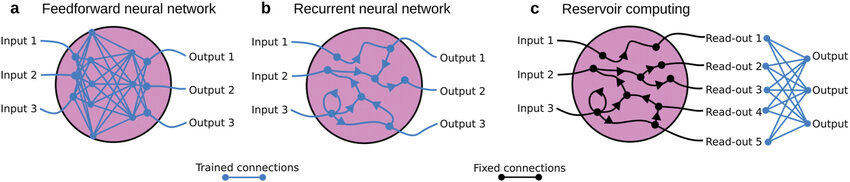
\includegraphics[width=\linewidth]{figures/rc_difference_with others.png}
    \column{0.5\textwidth}
    \begin{itemize}
      \item (a) Feedforward Neural Network (FNN): acyclic, all connections trained.
      \item (b) Recurrent Neural Network (RNN): cyclic, all connections trained.
      \item (c) Reservoir Computing: only output weights trained.
    \end{itemize}
  \end{columns}
\end{frame}

% Basics of Reservoir Computing
\section{Basics of Reservoir Computing}
\begin{frame}{General Principle}
  \begin{itemize}
    \item RC transforms input signals via a high-dimensional nonlinear reservoir.
    \item Only the output layer is trained; reservoir connections are fixed and random.
    \item Workflow:
      \begin{itemize}
        \item Input Layer: fixed random weights
        \item Reservoir: high-dimensional, recurrent, fixed
        \item Output Layer: trained linear readout
      \end{itemize}
  \end{itemize}
\end{frame}

\begin{frame}{Reservoir Computing Dynamics}
  \[
    \mathbf{x}[n+1] = f\bigl(\mathbf{W}\mathbf{x}[n] + \mathbf{W}^{\mathrm{in}}\mathbf{u}[n] + \mathbf{b}\bigr)
  \]
  \[
    \mathbf{y}[n] = \mathbf{W}^{\mathrm{out}}\bigl[\mathbf{x}[n];\,\mathbf{u}[n]\bigr]
  \]
  \begin{itemize}
    \item $\mathbf{x}[n]$: reservoir state
    \item $\mathbf{u}[n]$: input
    \item $\mathbf{W}$: fixed random weights
    \item $\mathbf{W}^{\mathrm{out}}$: trainable output weights
  \end{itemize}
\end{frame}

\begin{frame}{Physical Reservoir Computing}
  \begin{itemize}
    \item RC can use physical systems as reservoirs (optical, mechanical, spintronic, etc.).
    \item Exploits inherent nonlinearity and memory of physical substrates.
    \item Example: Single pendulum as a reservoir.
  \end{itemize}
\end{frame}

\begin{frame}{Echo State Property and Fading Memory}
  \begin{itemize}
    \item Echo State Property (ESP): Reservoir state depends only on input history, not initial state.
    \item Achieved by setting spectral radius of $\mathbf{W}$ less than one.
    \item Fading memory: Recent inputs have more influence; older inputs fade.
    \item Trade-off between memory capacity and nonlinearity.
  \end{itemize}
\end{frame}

\begin{frame}{Comparison with Traditional RNNs}
  \begin{itemize}
    \item \textbf{RNNs:} All weights trained via backpropagation through time (BPTT).
    \item \textbf{RC:} Only output weights trained (linear regression); input and recurrent weights fixed.
    \item Avoids vanishing/exploding gradients and reduces computational cost.
  \end{itemize}
\end{frame}

\begin{frame}{RC Variants: ESN and LSM}
  \begin{columns}
    \column{0.5\textwidth}
    \textbf{Echo State Networks (ESN):}
    \begin{itemize}
      \item Continuous activation (e.g., tanh)
      \item Sparse random connectivity
    \end{itemize}
    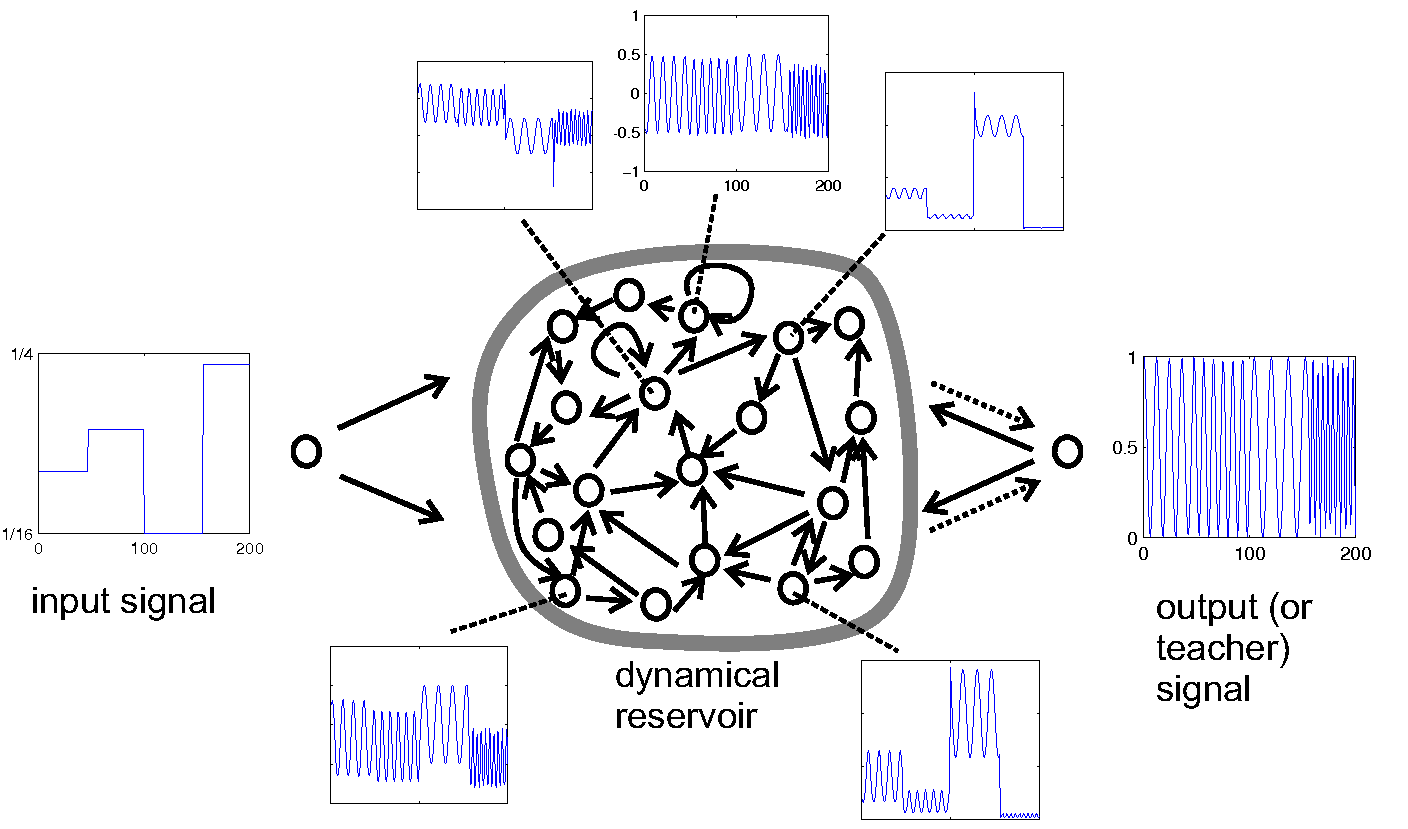
\includegraphics[width=\linewidth]{figures/ESN_diag_FreqGenSchema.png}
    \column{0.5\textwidth}
    \textbf{Liquid State Machines (LSM):}
    \begin{itemize}
      \item Spiking neuron models
      \item Inspired by biological neurons
    \end{itemize}
    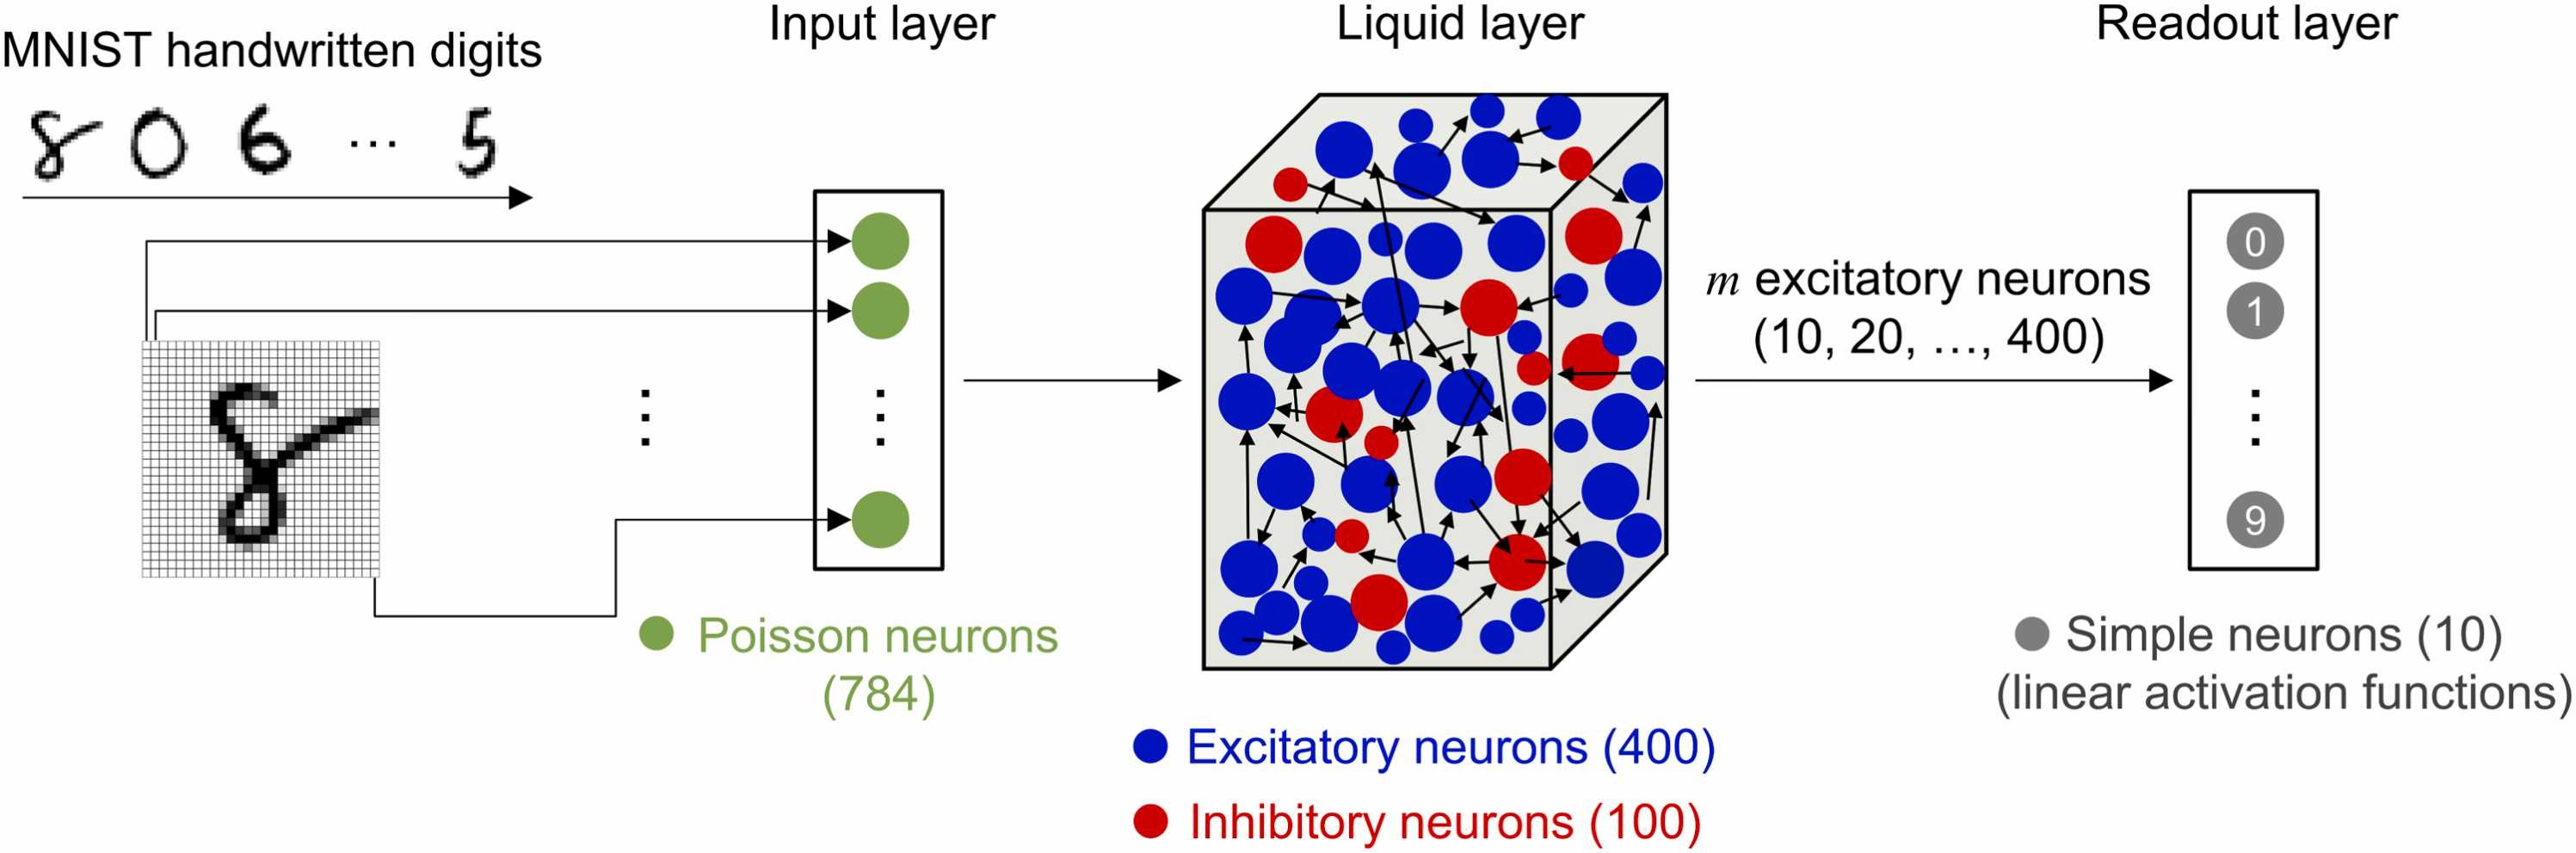
\includegraphics[width=\linewidth]{figures/lsm_diag.png}
  \end{columns}
\end{frame}

\begin{frame}{Physical Reservoir Computing (PRC)}
  \begin{itemize}
    \item RC can be implemented in physical media (e.g., pendulum, electronic circuits).
    \item Leverages real-world nonlinear dynamics for computation.
  \end{itemize}
\end{frame}

\begin{frame}{Training Methodology}
  \begin{enumerate}
    \item Feed input signals, collect reservoir states.
    \item Train linear readout (ridge regression) to map states to outputs.
    \item Apply trained readout to new data.
  \end{enumerate}
  \[
    W_{\text{out}} = YG^T\left(GG^T + \lambda I\right)^{-1}
  \]
  \begin{itemize}
    \item $Y$: target outputs, $G$: reservoir states, $\lambda$: regularization.
  \end{itemize}
\end{frame}

\begin{frame}{Advantages and Limitations}
  \textbf{Advantages:}
  \begin{itemize}
    \item Simple, fast training (linear regression).
    \item Same reservoir usable for multiple tasks.
    \item Amenable to physical implementation.
  \end{itemize}
  \vspace{0.2cm}
  \textbf{Limitations:}
  \begin{itemize}
    \item Limited control over function via random initialization.
    \item Memory capacity limited by reservoir size.
    \item Task performance depends on reservoir dynamics and hyperparameters.
  \end{itemize}
\end{frame}

% Literature Review
\section{Literature Review}
\begin{frame}{Literature Review: Key Studies}
  \begin{itemize}
    \item \textbf{Cucchi et al. (2022):} RC experiment setup and advantages.
    \item \textbf{Zhang \& Cornelius (2023):} RC limitations; “Catch-22s” in multistable systems.
    \item \textbf{Arun et al. (2024):} Logistic map as reservoir, robust to noise.
    \item \textbf{Mandal et al. (2022):} Physical reservoir using a pendulum.
    \item \textbf{Itoh et al. (2020):} Bifurcation diagram reconstruction via ELM.
  \end{itemize}
\end{frame}

% Implementation and Results
\section{Implementation and Results}
\begin{frame}{Pendulum Reservoir: Setup}
  \begin{itemize}
    \item Simulated a driven damped pendulum as reservoir.
    \item State vector: angle $x(t)$ and angular velocity $v(t)$.
    \item Dynamics:
      \[
      \begin{aligned}
      \frac{dx}{dt} &= v, \\
      \frac{dv}{dt} &= -\frac{g}{l} \sin(x) - k v + f\, \text{sign}(\sin(\omega t))
      \end{aligned}
      \]
  \end{itemize}
\end{frame}

\begin{frame}{Pendulum Reservoir: Results}
  \begin{itemize}
    \item Trained output layer to predict target time series.
    \item Demonstrated learning of time-dependent tasks.
  \end{itemize}
  \begin{center}
    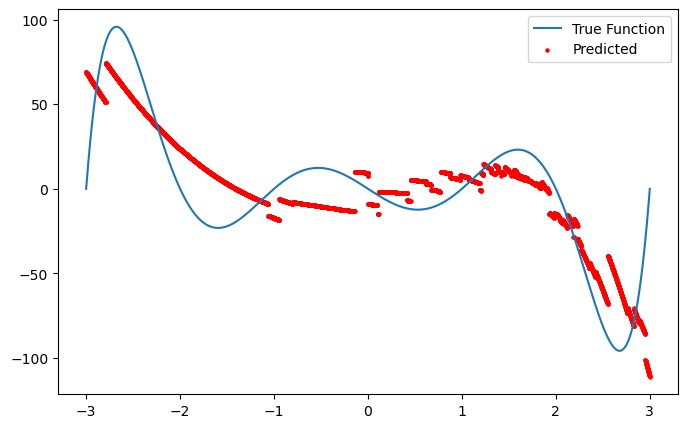
\includegraphics[width=0.75\linewidth]{figures/pendulum_result_0.png}
  \end{center}
\end{frame}

\begin{frame}{Lorenz System Prediction (Pendulum Reservoir)}
  \begin{itemize}
    \item Lorenz system:
      \[
      \begin{aligned}
      \frac{dx}{dt} &= \sigma (y - x), \\
      \frac{dy}{dt} &= x (\rho - z) - y, \\
      \frac{dz}{dt} &= x y - \beta z
      \end{aligned}
      \]
    \item Used $x$ as input, predicted $(x, y, z)$.
  \end{itemize}
\end{frame}

\begin{frame}{Lorenz: Actual vs Predicted}
  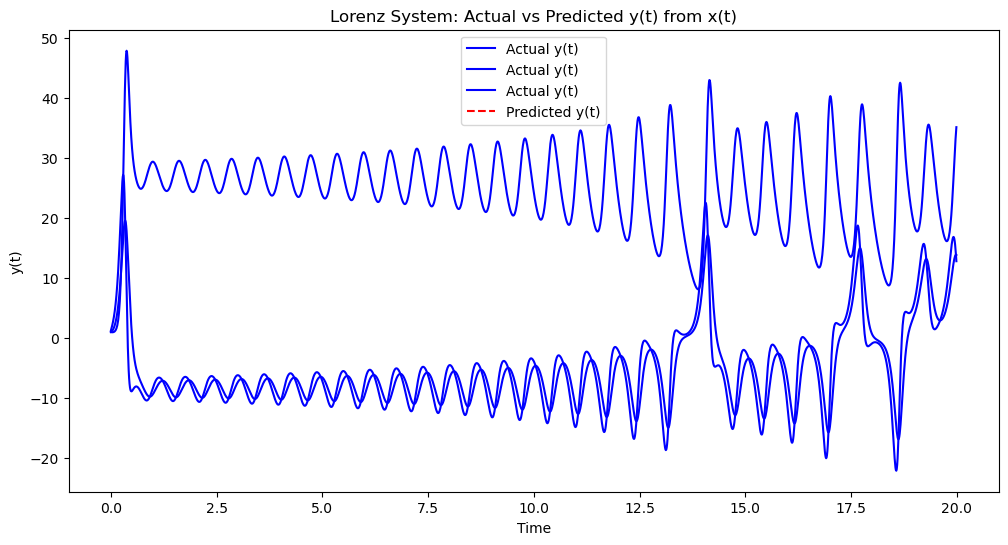
\includegraphics[width=1\linewidth]{figures/lorentz_pendulum_1.png}
\end{frame}

\begin{frame}{Lorenz: 3D Trajectory}
  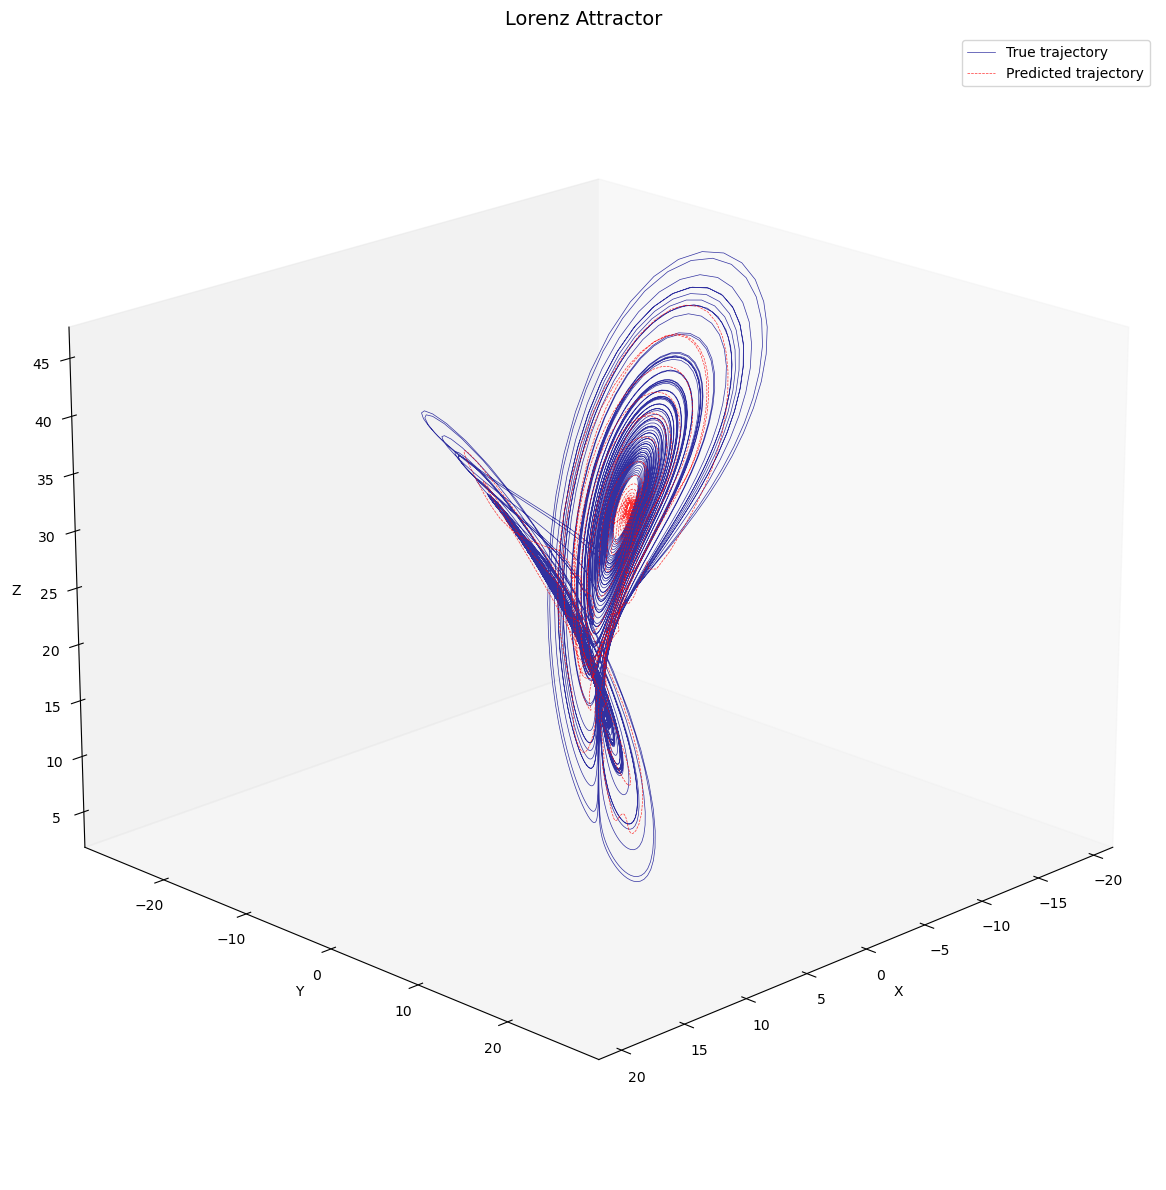
\includegraphics[width=1\linewidth]{figures/lorentz_pendulum_2.png}
\end{frame}

\begin{frame}{Logistic Map Reservoir}
  \begin{itemize}
    \item Logistic map: $x_{n+1} = r x_n (1-x_n)$.
    \item Used virtual nodes for high-dimensional reservoir.
    \item Benchmarked with 7th-degree polynomial.
  \end{itemize}
  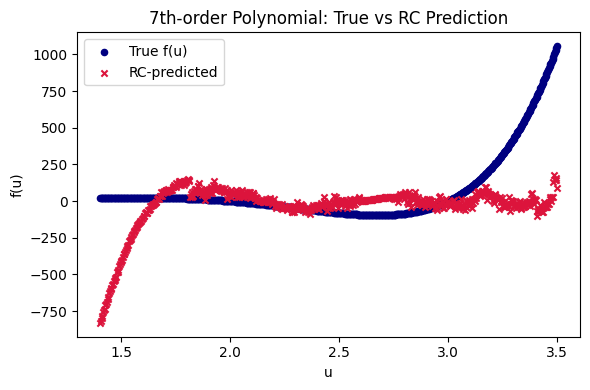
\includegraphics[width=0.75\linewidth]{figures/logistic_7th_degree.png}
\end{frame}

\begin{frame}{Lorenz Prediction (Logistic Map Reservoir)}
  \begin{itemize}
    \item Test RMSE (x, y, z): [3.77, 2.94, 8.36]
  \end{itemize}
  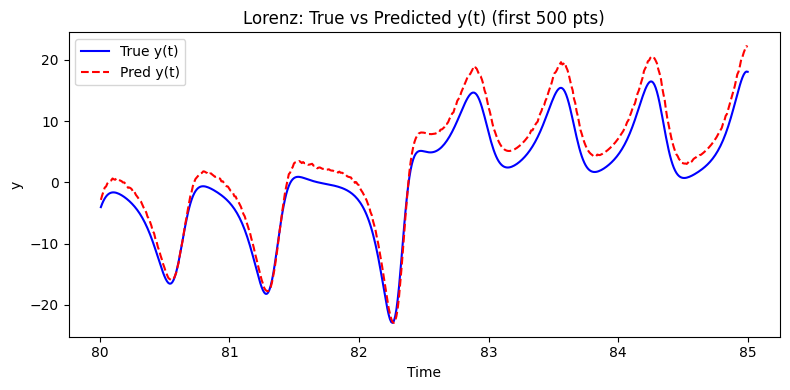
\includegraphics[width=1\linewidth]{figures/lorentz_logistic_pred_true.png}
\end{frame}

\begin{frame}{Lorenz: Axis Evolution (Logistic Map Reservoir)}
  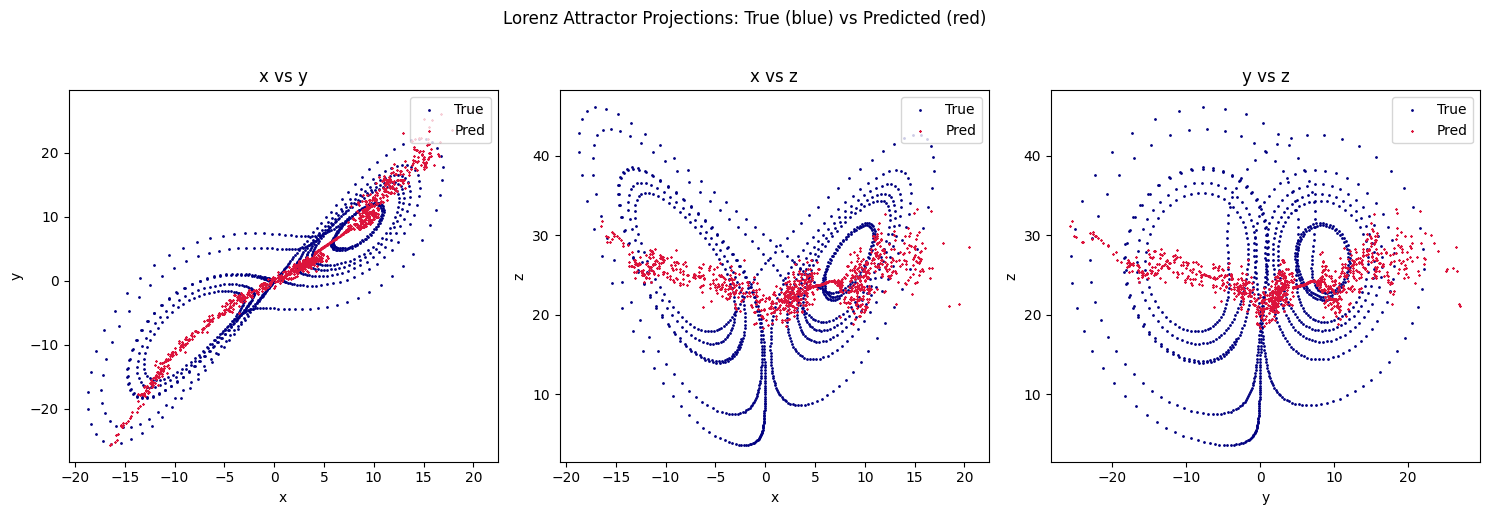
\includegraphics[width=1\linewidth]{figures/lorenz_logistic_pred_diagram.png}
\end{frame}

\begin{frame}{Bifurcation Reconstruction via PCA and ELM}
  \begin{itemize}
    \item Simulate system for parameter range $\mu$.
    \item Collect reservoir states, apply PCA.
    \item Train ELM to map PCA features + $\mu$ to output.
    \item Sweep $\mu$ to reconstruct bifurcation diagram.
  \end{itemize}
\end{frame}

\begin{frame}{Bifurcation Diagram: Initial Attempt}
  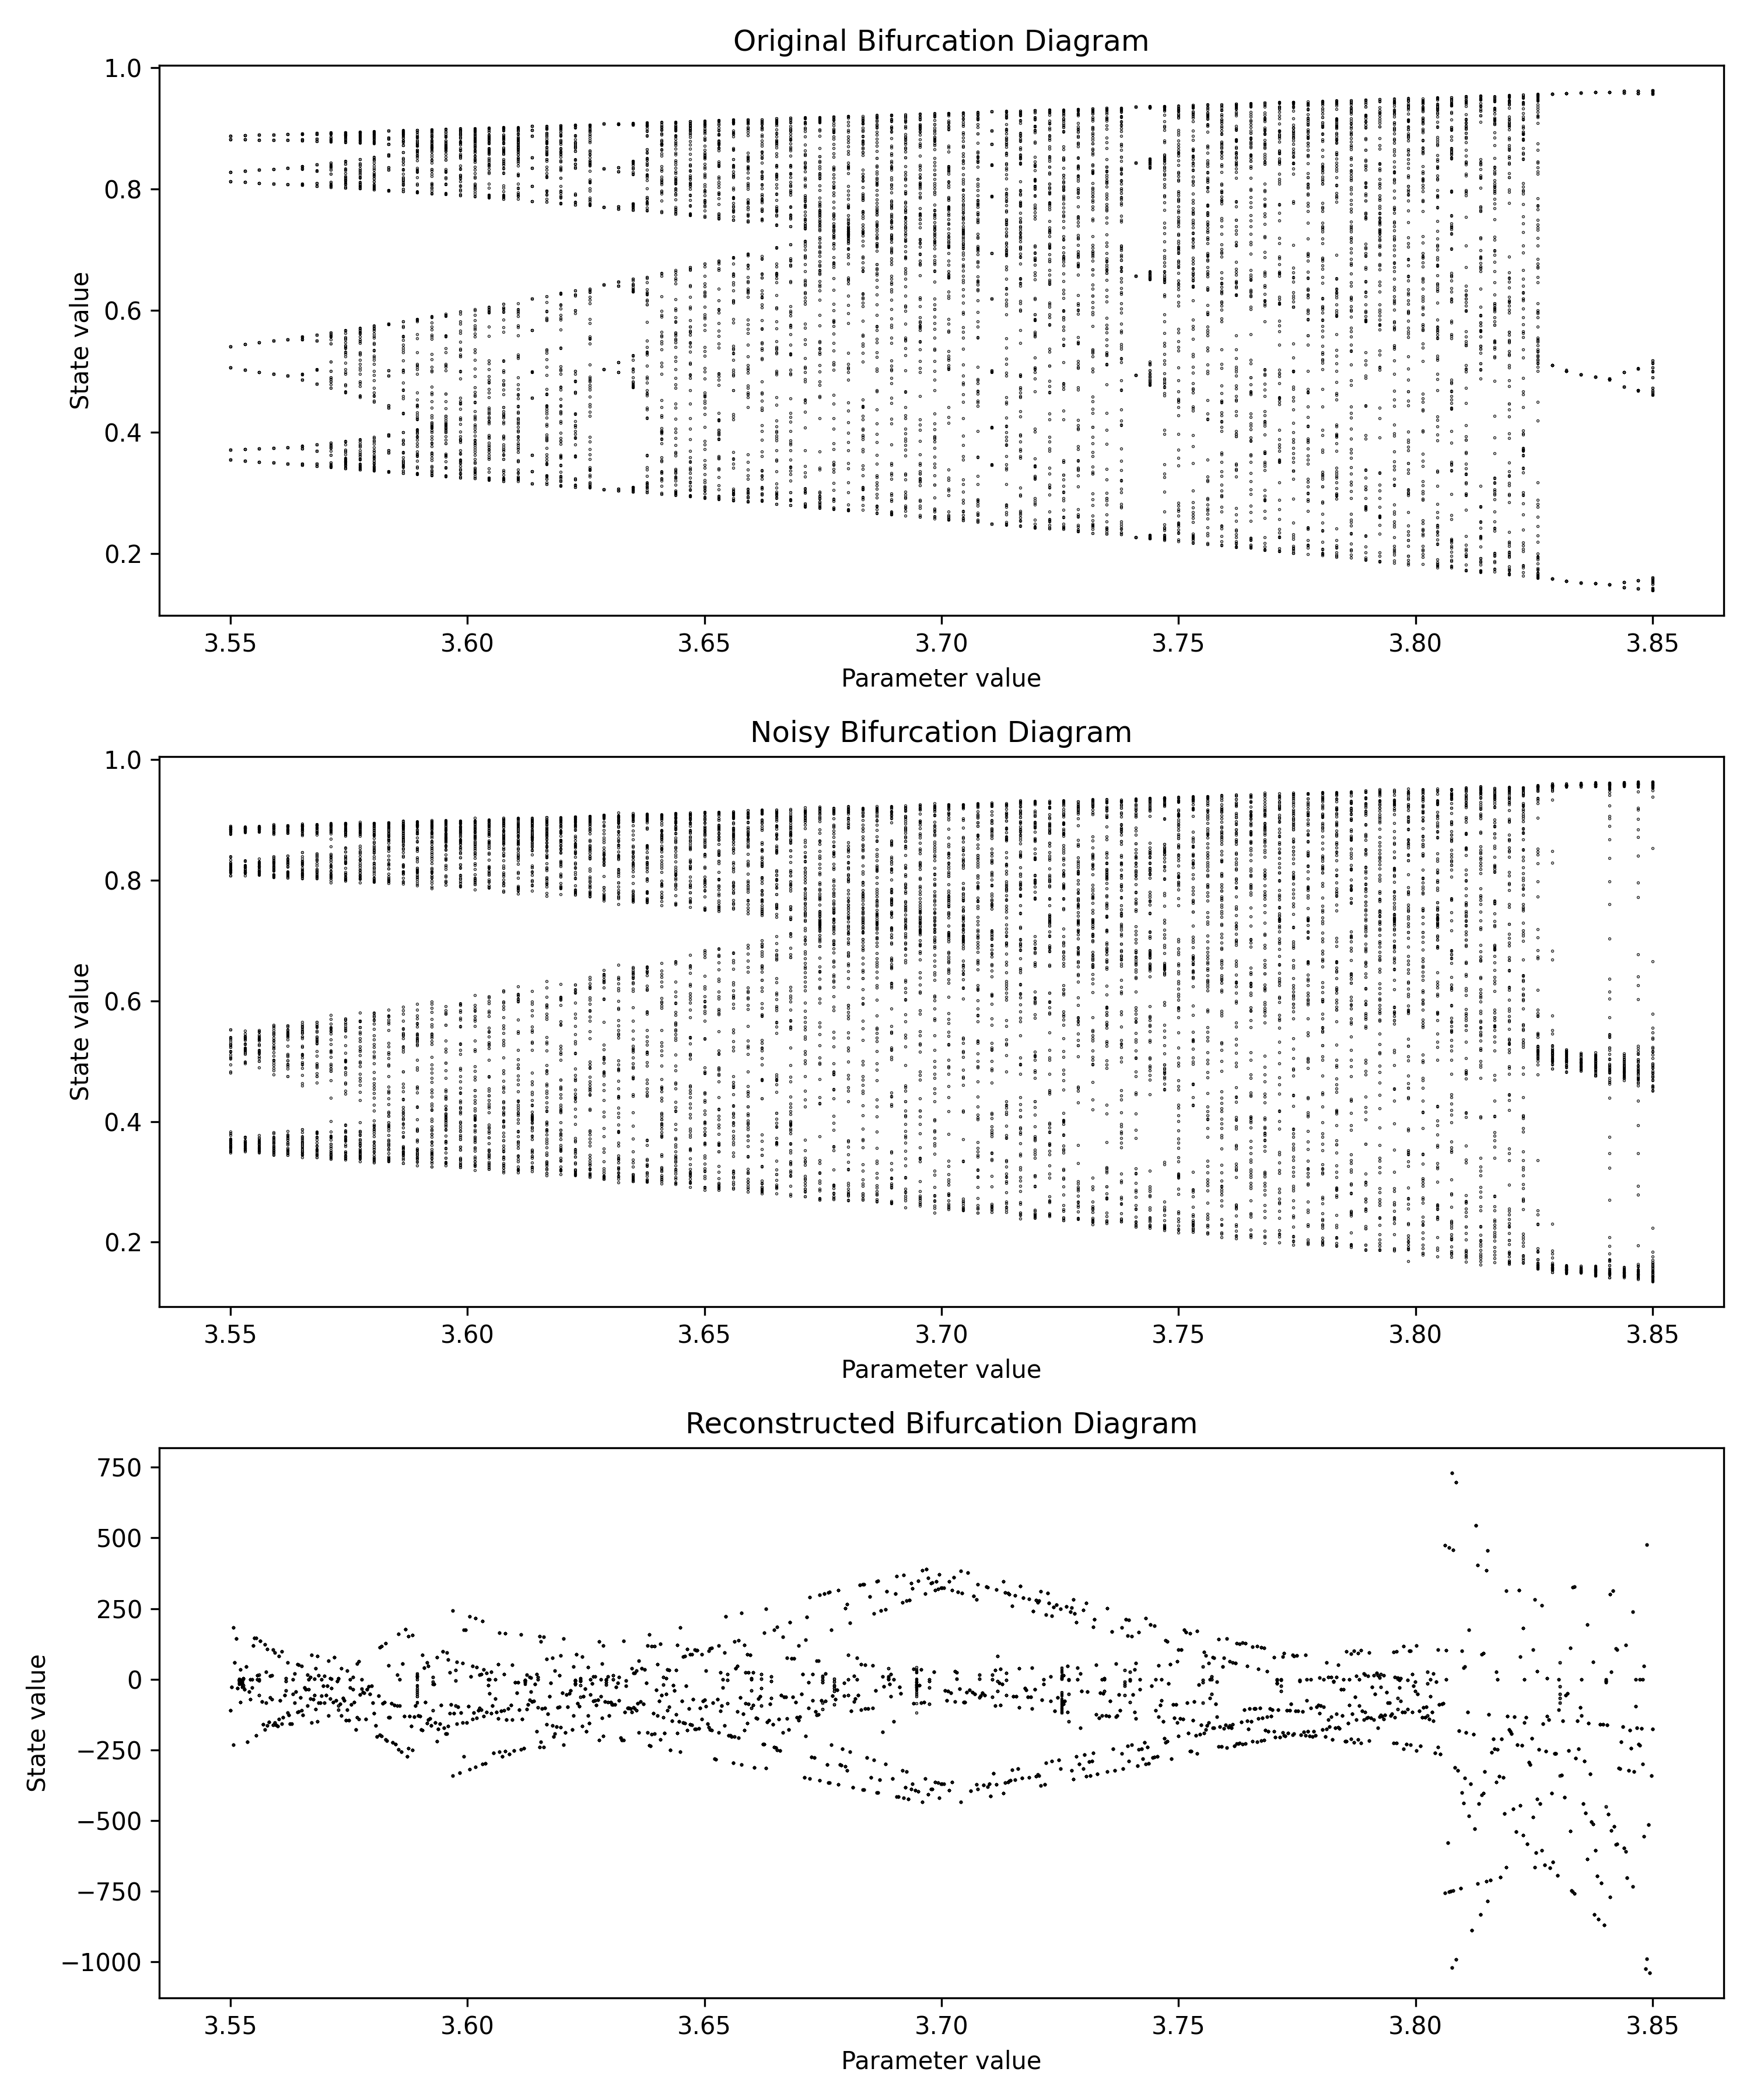
\includegraphics[width=1\linewidth]{figures/bd_reconstruction_elm.png}
\end{frame}

\begin{frame}{Bifurcation Diagram: Improved Results}
  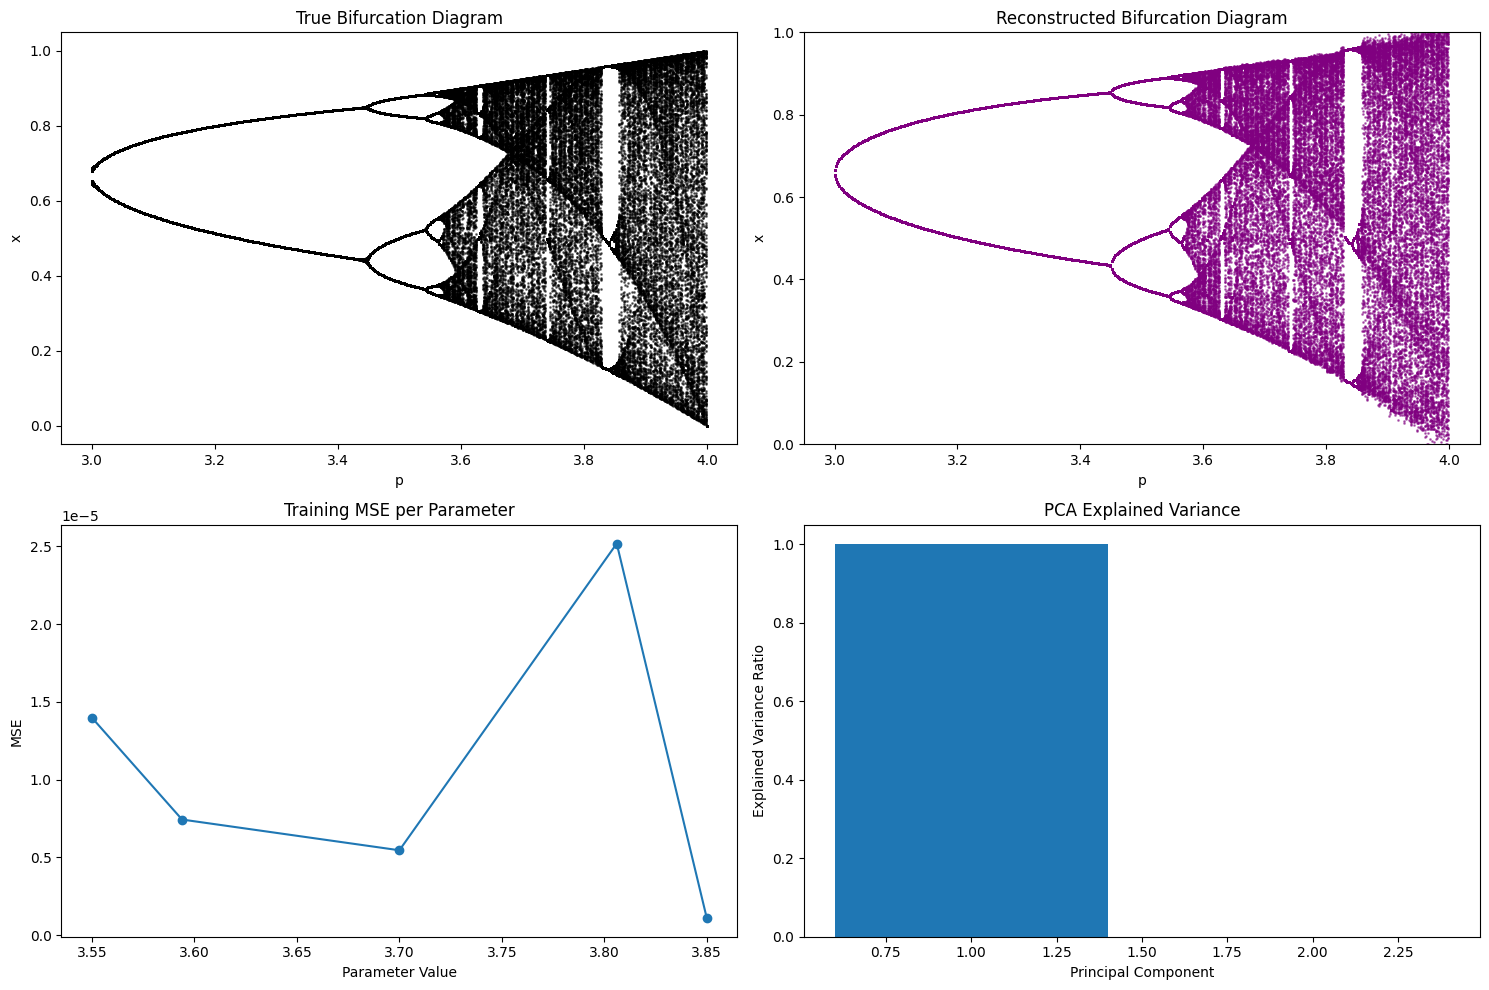
\includegraphics[width=1\linewidth]{figures/bd_1_results.png}
\end{frame}

\begin{frame}{Return Plot Reconstruction}
  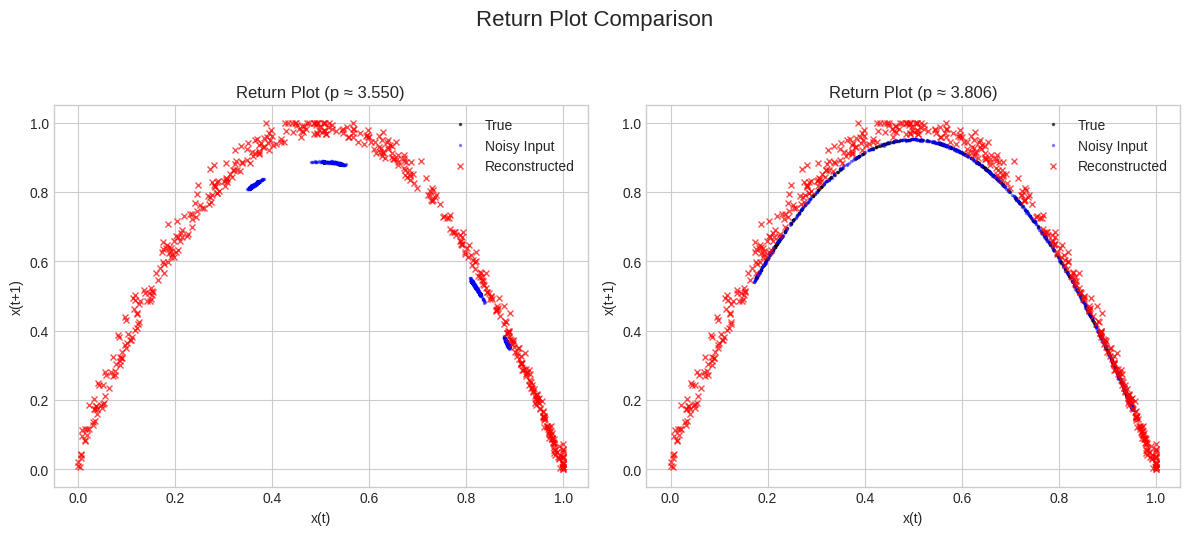
\includegraphics[width=1\linewidth]{figures/bd_return_plot_2.png}
\end{frame}

\begin{frame}{True vs Predicted Bifurcation}
  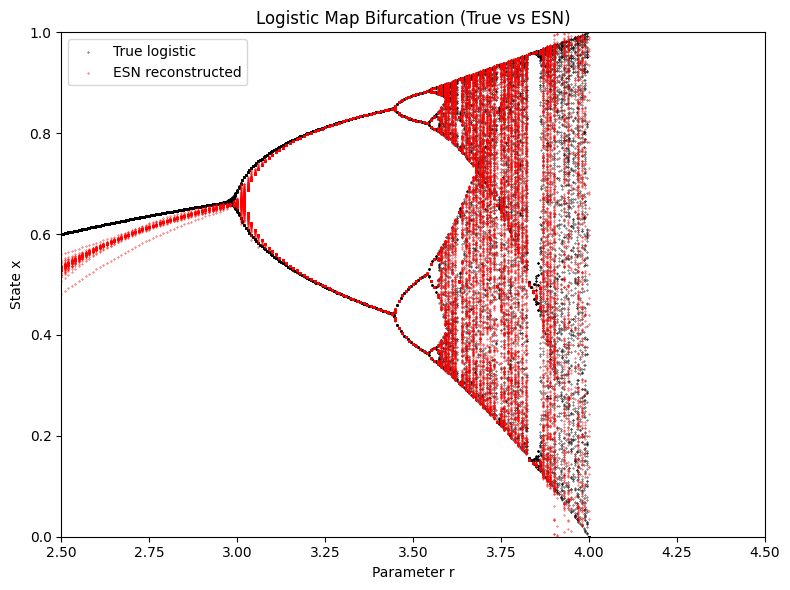
\includegraphics[width=0.8\linewidth]{figures/bf_3_results_overlapped.png}
\end{frame}

\begin{frame}{Lyapunov Exponent Estimation}
  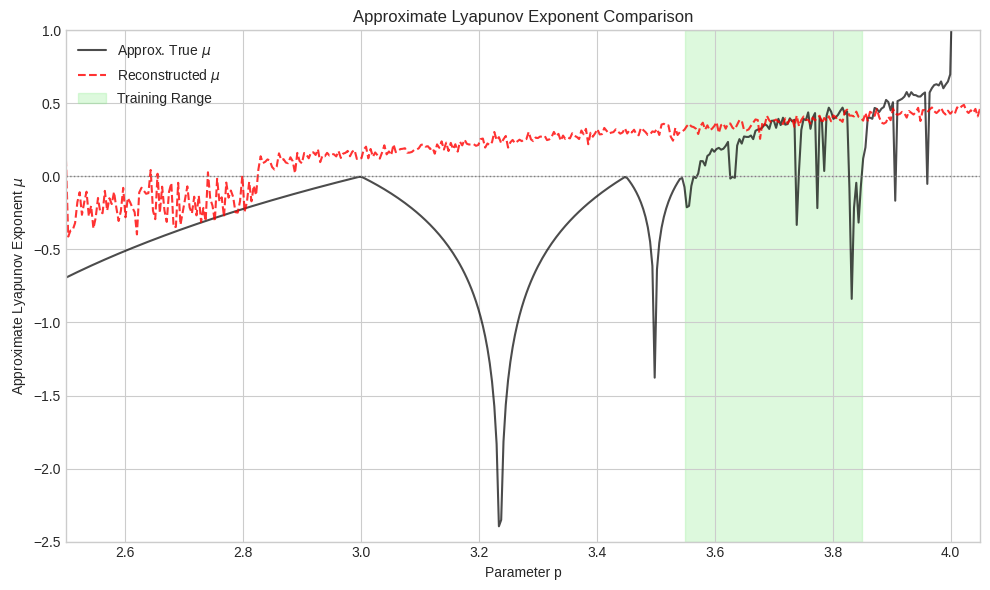
\includegraphics[width=1\linewidth]{figures/lyapanov_bd_rd.png}
\end{frame}

\begin{frame}{PCA Component Analysis}
  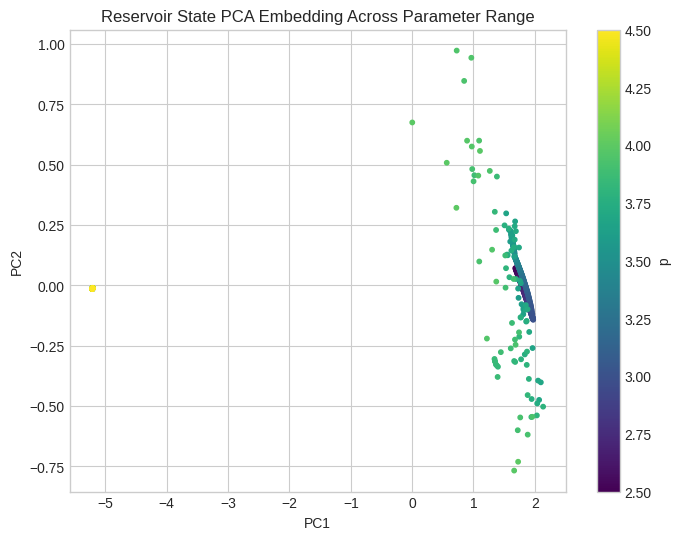
\includegraphics[width=0.8\linewidth]{figures/bd_elm_pca_analysis.png}
\end{frame}

\begin{frame}{Prediction for Specific Parameter}
  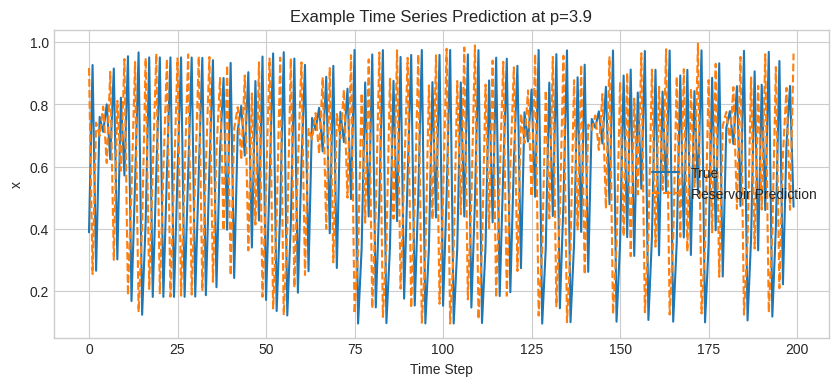
\includegraphics[width=1.0\linewidth]{figures/bd_5_prediction_for_specific_value.png}
\end{frame}

\begin{frame}{Using Recurrent Networks (LSTM)}
  \begin{itemize}
    \item LSTM receives $(x_t, p)$ as input, predicts $x_{t+1}$:
      \[
        \hat{x}_{t+1} = g_{\text{LSTM}}(x_t, p; \theta)
      \]
    \item Trained on all parameters; learns conditional dynamics.
    \item Outperforms RC for bifurcation reconstruction.
  \end{itemize}
  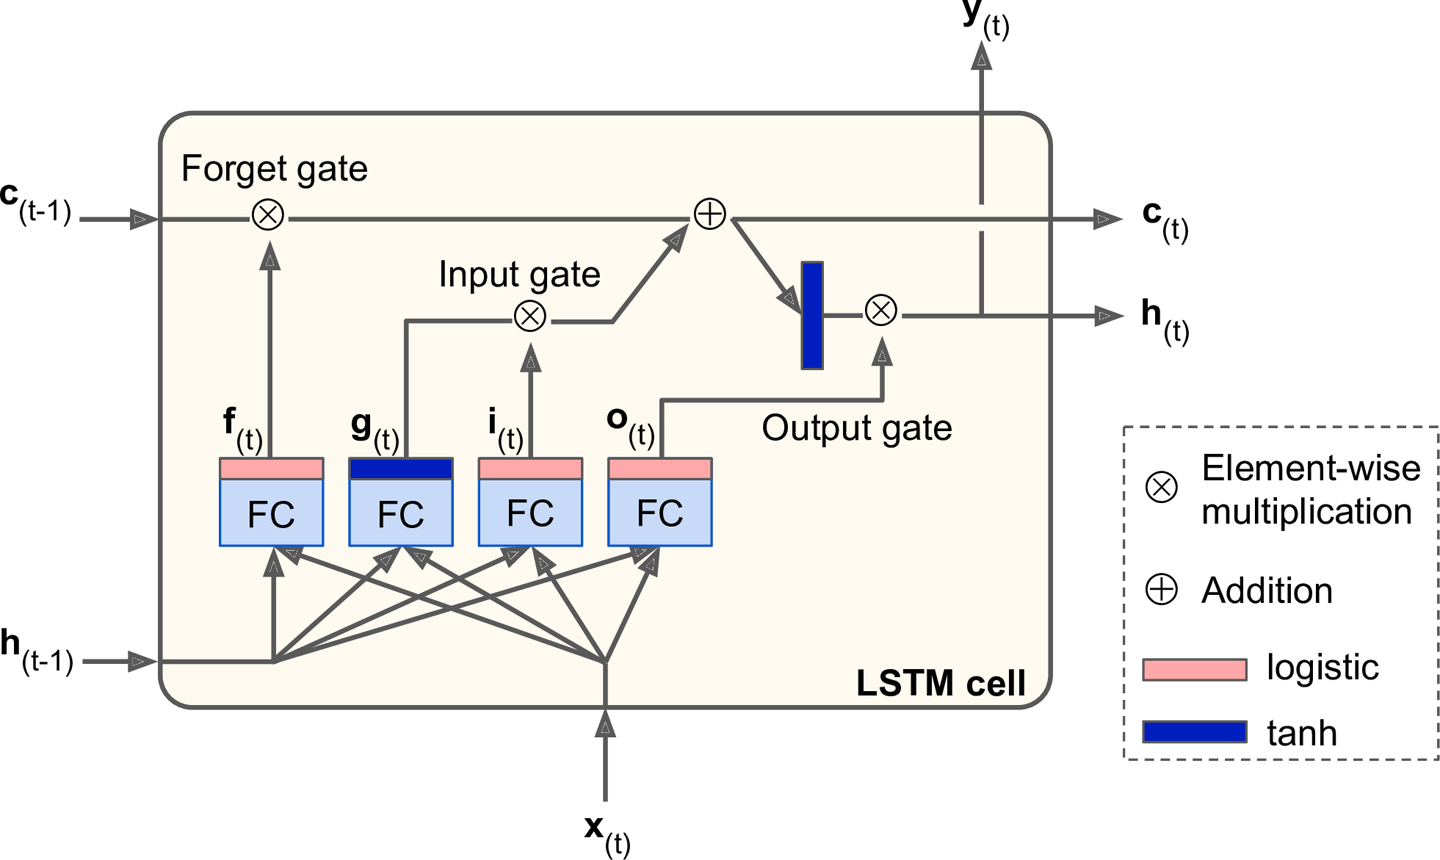
\includegraphics[width=1\linewidth]{figures/LSTM_arch.png}
\end{frame}

\begin{frame}{LSTM: Bifurcation Diagram Reconstruction}
  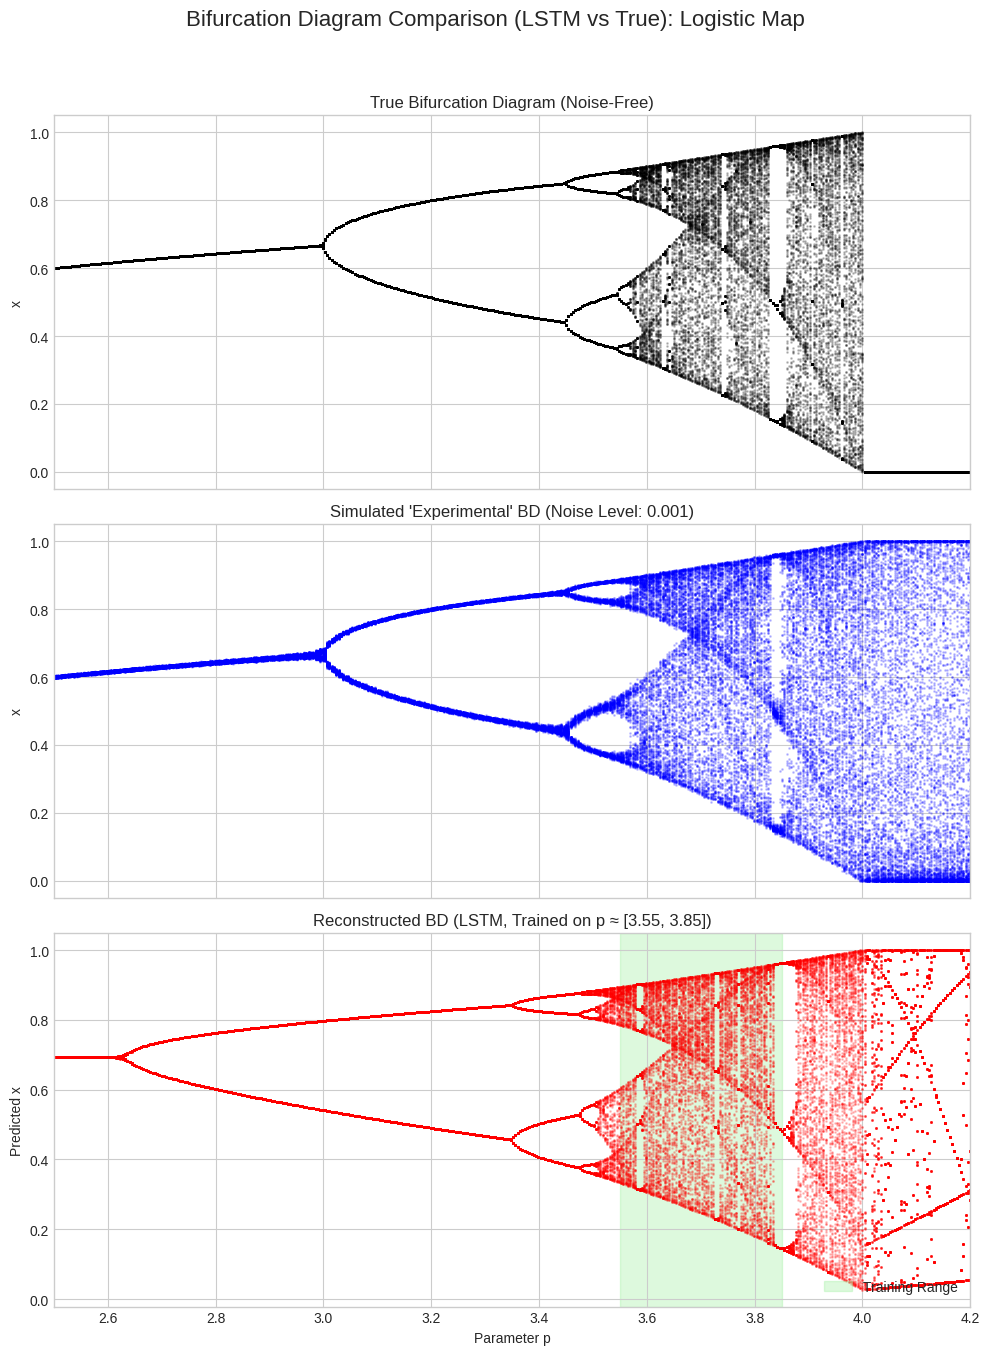
\includegraphics[width=1.0\linewidth]{figures/lstm_bd_1.png}
\end{frame}

\begin{frame}{LSTM: Return Plot Reconstruction}
  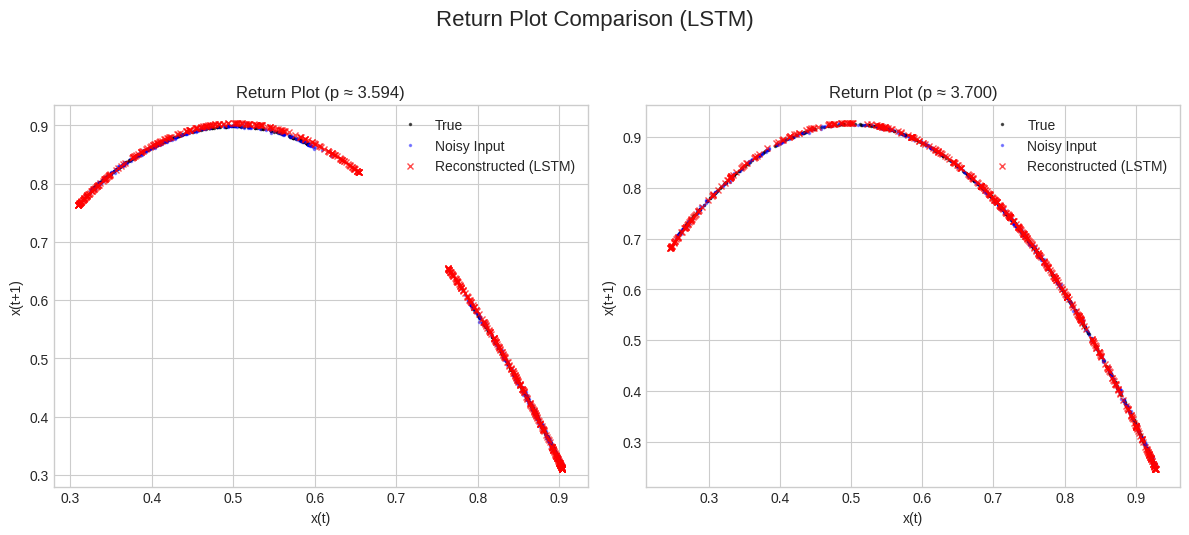
\includegraphics[width=1.0\linewidth]{figures/lstm_bd_2.png}
\end{frame}

\begin{frame}{LSTM: Lyapunov Exponent Estimation}
  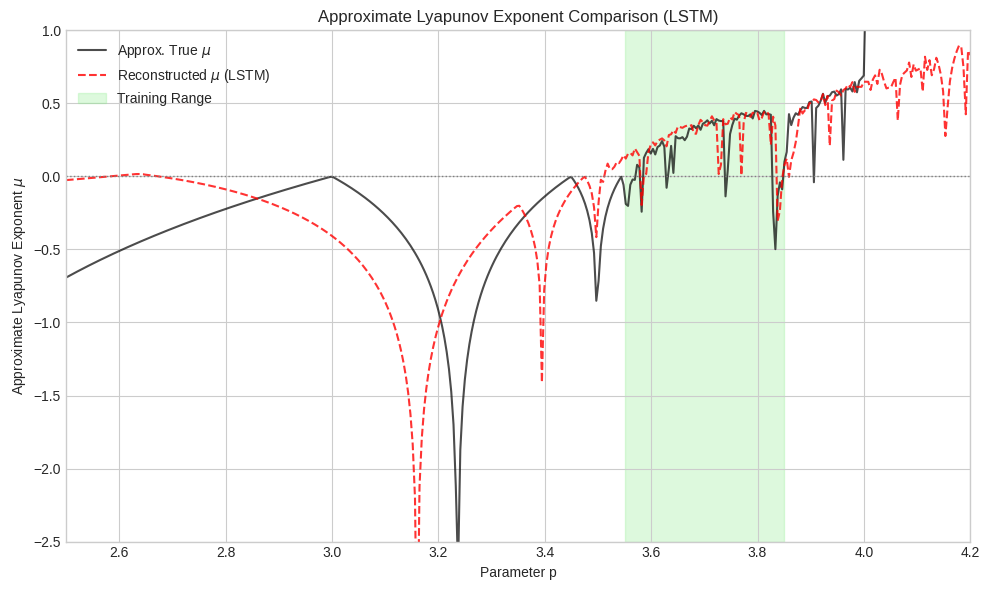
\includegraphics[width=1.0\linewidth]{figures/lstm_bd_3.png}
\end{frame}

\begin{frame}{RC vs LSTM: Training Time}
  \begin{itemize}
    \item LSTM: $\sim$46 seconds to train.
    \item ELM (RC): $<$1 second.
    \item RC is efficient for training, but LSTM offers better flexibility and extrapolation.
  \end{itemize}
\end{frame}

% Conclusion
\section{Conclusion}
\begin{frame}{Conclusion}
  \begin{itemize}
    \item RC enables efficient modeling of temporal data with minimal training.
    \item Successfully reconstructed broad bifurcation features; struggled with fine structure and extrapolation.
    \item LSTM and other RNNs may be better for complex dynamics, given modern computational resources.
  \end{itemize}
\end{frame}

\begin{frame}{Future Work}
  \begin{itemize}
    \item Optimize RC hyperparameters (size, spectral radius, etc.).
    \item Apply to more systems: higher-dimensional, continuous-time, coupled.
    \item Compare with deep RC, alternative readouts.
    \item Validate on physical hardware data.
  \end{itemize}
\end{frame}

\begin{frame}{Acknowledgement}
  I would like to thank \textbf{Prof. Gaurav Dar} for his guidance, insights, and motivation throughout this project.
\end{frame}

\end{document}
